\documentclass{jlreq}

\usepackage{amsmath}
\usepackage{array}
\usepackage{bm}
\usepackage{caption}
\usepackage{fancyhdr}
\usepackage{float}
\usepackage{graphicx}
\usepackage{listings}
\usepackage{multirow}
\usepackage{physics}
\usepackage{siunitx}
\usepackage{xcolor}

\lstset{
    language=Verilog, % 使用するプログラム言語を指定
    basicstyle=\ttfamily\footnotesize, % フォントの指定
    tabsize=4, % インデント幅
    numbers=left, % 行番号を表示(必要な場合)
    numberstyle=\tiny, % 行番号のスタイル
    frame=single, % ソースコードを枠で囲む(必要な場合)
    breaklines=true, % 長い行を自動的に折り返す
    captionpos=t, % キャプションの位置を上にする
    showstringspaces=false, % 文字列内のスペースを表示しない
    keywordstyle=\color{blue}, % キーワードの色
    commentstyle=\color{green}, % コメントの色
    stringstyle=\color{red}, % 文字列の色
}
\renewcommand{\lstlistingname}{ソースコード}

\numberwithin{equation}{section}

\pagestyle{fancy}
\fancyhf{}
\fancyhead[R]{\thepage}

\begin{document}

\tableofcontents
\clearpage

\section{実験の目的}
算術演算を行うための論理回路について学ぶ.一般に,コンピュータ内では数を2進数で表現するため,
2進数に対する算術演算が行われる.論理回路の観点からこの算術演算について眺めると,その基本は1ビットの加算回路にある.
本実習では,加減算器および乗算器を設計する.

\section{実験器具}
実験に用いた環境を以下に示す.
\begin{description}
  \item[PC] Inspiron 15 3535
  \item[OS] Windows11
  \item[CPU] AMD Ryzen 5 7530U with Radeon Graphics 2.00 GHz
  \item[統合開発環境] Quartus Prime Lite Edition Version 20.1.1
  \item[FPGAボード] Terasic DE1SoC
\end{description}

\section{理論}
\subsection{全加算器}
2つの2進数の和を計算する回路を半加算器(half adder)と呼ぶ.さらに,下の桁からの桁上げ(キャリ; carry)を考慮して2つの2進数の和を計算する回路を全加算器(full adder; FA)と呼ぶ.

表\ref{tab:full_adder_table}に1ビットの全加算器の真理値表を示す.AとBが被加数と加数の入力で,$\text{C}_{in}$が下の桁からの桁上げ入力(キャリイン; carry-in)を表す.
また,Sはその桁の和の値であり,$\text{C}_{out}$は上の桁への桁上げ出力(キャリアウト; carry-out)を表す.この全加算器は組み合わせ回路で構成することができる.
\begin{table}[H]
  \centering
  \caption{1ビット全加算器の真理値表}
  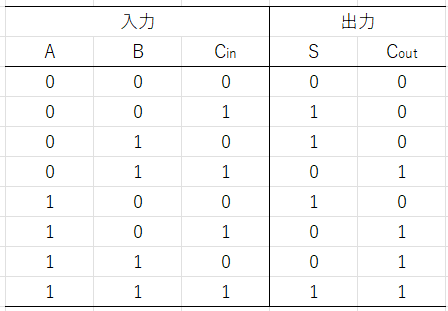
\includegraphics{assets/full_adder_table.png}
  \label{tab:full_adder_table}
\end{table}

\subsection{補数と減算}
2進数で負の数を表現する方式にはいくつかの方式があるが,一般には2の補数表現(two's complement)が用いられる.
符号ビットは,値が0または正のとき0とし,負のときには1と定める.符号の反転,は元の値が正か負かにかかわらず,各ビットを反転させて1を加えるという
同一の手続きによって行うことができる.2の補数表現で表現された2つの値を加算する場合には,それらを符号なし整数とみなして加算を行い,最上桁からの桁上げが生じても無視すればよい.

\subsection{加減算器の設計}
図\ref{fig:4bit_ripple_carry_adder}に4bitリプルキャリ加算器の回路を示す.この回路では,2個の4ビット値$A$($[A_3A_2A_1A_0]$)と$B$($[B_3B_2B_1B_0]$)を加算し,
和$S$($[S_3S_2S_1S_0]$)を求めている.この方式では,下位ビット(図の右側)から全加算器(図中ではFAと表現)で加算を行い,桁上げ(キャリ)が生じた場合は上位ビットに伝達する.
キャリが波(リプル; ripple)のように伝搬することからリプルキャリ方式と呼ばれる.
\begin{figure}
  \centering
  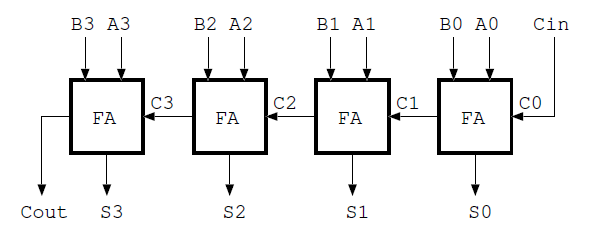
\includegraphics{assets/4bit_ripple_carry_adder.png}
  \caption{4bitリプルキャリ加算器}
  \label{fig:4bit_ripple_carry_adder}
\end{figure}

図\ref{fig:8bit_signed_addsub}のAddSubは8ビット符号付き加減算器を示している.2の補数表現で表される8ビット値Aを入力し,前回の結果にAを加減算した結果をSとして出力する.
AddSubは1ビットの命令入力信号MODEを持ち,MODE=0のときは加算($S+A$),MODE=1のときは減算($S-A$)を行うものとする.
1ビット出力OFはオーバーフロー(overflow; 桁あふれ)を表しており,Sが正しい符号付き値ではない場合に1にする.
\begin{figure}[H]
  \centering
  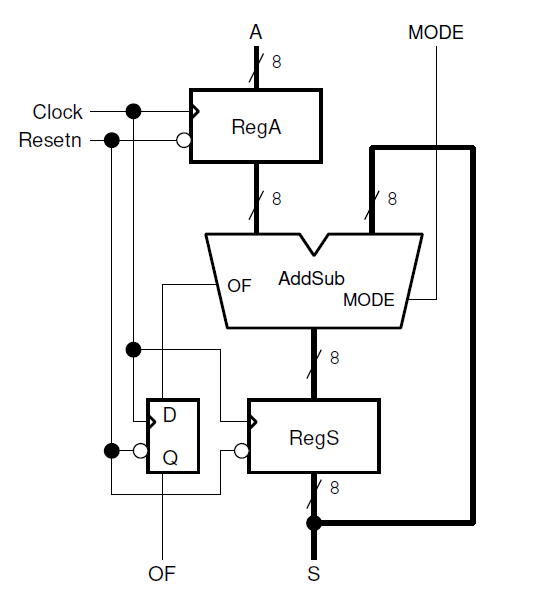
\includegraphics{assets/8bit_signed_adder_subtractor.png}
  \caption{8ビット符号付き加減算器}
  \label{fig:8bit_signed_addsub}
\end{figure}

図\ref{fig:8bit_signed_addsub}では,Aの値を一度8ビット幅のレジスタRegAに保持してから,AddSub部に供給している.
同様に,AddSub部からの出力をレジスタRegSで受けている.これらのレジスタにはリセット入力を接続し,任意のタイミングで0にできるようにしている.

\subsection{信号遅延の問題}
実際の回路ではAND,OR,NOTなどの回路素子を通過するごとに遅延が生じる.図\ref{fig:logic_delay}はNOT素子における信号遅延の例を示しており,
入力がHighになってから一定の遅延時間の後に出力がLowに反転していることが分かる.
\begin{figure}[H]
  \centering
  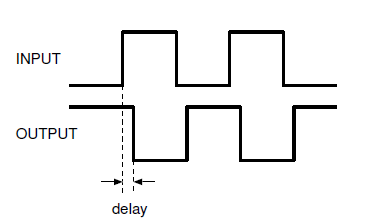
\includegraphics{assets/logic_delay.png}
  \caption{NOT素子における信号遅延}
  \label{fig:logic_delay}
\end{figure}
回路内部において,レジスタ間を伝搬する信号の経路(パス; path)のうち,遅延時間が最も大きい経路をクリティカルパス(critical path)という.
クリティカルパスにおける遅延時間がクロック同期を下回れば,そのクロック周期で回路は正常に動作することになる.逆に遅延時間が上回ると誤動作が生じる可能性があるため,設計時には十分なタイミング解析を行う必要がある.

FPGA開発ツールでは,回路の設計者が指示する「タイミングに関する設計要求(タイミング制約; timing constraint)」を用いて,最終的な回路の最適化を行う.
タイミング解析の結果,タイミング制約の範囲内であれば回路は設計要求を満たしていると判断でき,逆にタイミング制約を満たさなければ,設計要求を満たしていないことになる.

\subsection{乗算器の設計}
ここでは4ビット乗算器を順序回路を用いて設計することを考える.乗算回路のブロック図を図\ref{fig:4bit_mul_circuit}に示す.
\begin{figure}[H]
  \centering
  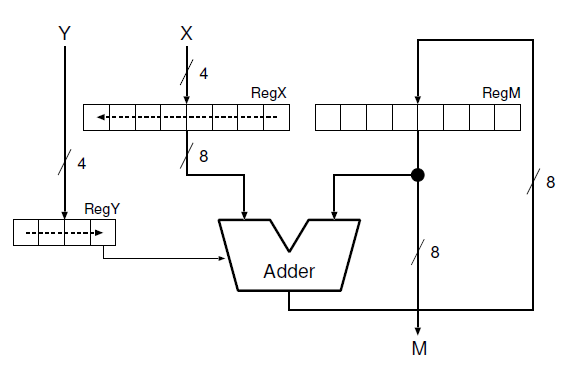
\includegraphics{assets/4bit_mul_circuit.png}
  \caption{4ビット乗算器のブロック図}
  \label{fig:4bit_mul_circuit}
\end{figure}
簡単のため,乗数と被乗数はどちらも4ビット符号なし数とし,被乗数を$X = [x_3x_2x_1x_0]$,乗数を$Y = [y_3y_2y_1y_0]$とした上で,乗算結果を8ビット符号なし整数$M$に格納するものとする.
このとき,積$M$を求める式は以下のように変形できる.
\begin{align}
  M & = X \cdot Y                                                                                             \\
    & = X \cdot (y_3 \cdot 2^3 + y_2 \cdot 2^2 + y_1 \cdot 2^1 + y_0 \cdot 2^0)                               \\
    & = y_3 \cdot (X \cdot 2^3) + y_2 \cdot (X \cdot 2^2) + y_1 \cdot (X \cdot 2^1) + y_0 \cdot (X \cdot 2^0)
\end{align}
最初に,$y_0 \cdot (X \cdot 2^0)$の部分積が求まれば,Yレジスタを1ビット右シフト,Xレジスタを1ビット左シフトする.すると,Yレジスタは$[0y_3y_2y_1]$となり,最下位ビットが$y_1$に変化する.
Xレジスタの内容も$[000x_3x_2x_1x_00]$になり,これは$X \cdot 2^1$の値である.あとは同様に,Yレジスタの最下位ビット$y_1$が1であればXレジスタの値をMレジスタの値に加算すればよい.以降は,この手順の繰り返しである.

\section{演習の解答}
\subsection{演習1}
実験テキストの表7の出力変数を入力変数の論理式として表したものを以下に示す.
\begin{align}
  S & = \bar{A} \bar{B} C_{in} + \bar{A} B \bar{C_{in}} + A \bar{B} \bar{C_{in}} + A B C_{in} \\
    & = (\bar{A}\bar{B} + AB)C_{in} + (\overline{A}B + A\overline{B})\overline{C_{in}}        \\
    & = \overline{(A \oplus B)}C_{in} + (A \oplus B)\overline{C_{in}}                         \\
    & = (A \oplus B) \oplus C_{in}
\end{align}
\begin{align}
  C_{out} & = \bar{A} B C_{in} + A \bar{B} C_{in} + A B \overline{C_{in}} + A B C_{in} \\
          & = (\bar{A} B + A \bar{B})C_{in} + AB(C_{in} + \overline{C_{in}})           \\
          & = (A \oplus B)C_{in} + AB
\end{align}

また,このときの回路図は図\ref{fig:enshu1}のようになる.
\begin{figure}[H]
  \centering
  
\includegraphics[width=\textwidth]{assets/enshu1.png}
  \caption{演習1の1ビット全加算器の回路図}
  \label{fig:enshu1}
\end{figure}

\subsection{演習2}
最大動作周波数の大小が関係しているのはクリティカルパスにかかる時間の大小であり,クリティカルパスの論理ゲートの段数が多いほど電気信号が通る時間がかかってしまう.
そのため,最大動作周波数を高めるにはクリティカルパスの段数を最小にするといった時間最適化を行えばよい.時間最適化の一例として,カルノー図による2段論理最小化が挙げられる.\cite{logical_circuit_text}

\subsection{演習3}
実験テキストの図42より,単純化が可能になるとしたらA0~A3の部分を簡略化することである.
A0からA3までのレジスタは同じ動作をし,Yが0になったときに計算結果がMに反映されるため,
図\ref{enshu4}のように単純化を行えばよい.
\begin{figure}[H]
  \centering
  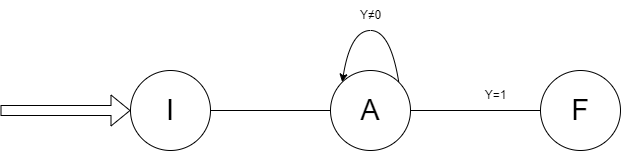
\includegraphics[width=\textwidth]{assets/enshu4.png}
  \caption{単純化した状態遷移図}
  \label{enshu4}
\end{figure}

\section{実習}
\subsection{実習1}
8ビット符号付き加減算器をリプルキャリ方式で行うように実装したVerilog HDLのコードをソースコード\ref{src:ripple_addsub}に示す.
また,下位モジュールについてはソースコード\ref{src:dff_with_bit_param}~\ref{src:1bit_full_adder}に示す.
\begin{lstlisting}[caption={8ビット符号付き加減算器の上位モジュール}, label={src:ripple_addsub}]
module ripple_addsubtractor(Clk, Resetn, MODE, A, S, OF);
	input Clk, Resetn, MODE;
	input [7:0] A;
	output [7:0] S;
	output OF;
	
	wire [7:0] RegA_out, AddSub_out, RegS_out;
	wire _OF;
	
	assign S = RegS_out;
	
	D_FF #(8) RegA(Clk, Resetn, A, RegA_out);
	AddSub iAddSub(RegA_out, RegS_out, MODE, AddSub_out, _OF);
	D_FF #(8) RegS(Clk, Resetn, AddSub_out, RegS_out);
	D_FF DFF_OF(Clk, Resetn, _OF, OF);
endmodule
\end{lstlisting}

\begin{lstlisting}[caption={ビット幅をパラメータに持つDFFモジュール}, label={src:dff_with_bit_param}]
module D_FF(Clk, Resetn, D, Q);
	parameter bitwidth = 1;
	
	input Clk, Resetn;
	input [bitwidth-1:0] D;
	output reg [bitwidth-1:0] Q;
	
	always @(posedge Clk or negedge Resetn) begin
		if(!Resetn)
			Q <= 0;
		else
			Q <= D;
	end
endmodule
\end{lstlisting}

\begin{lstlisting}[caption={AddSubの動作をするモジュール}, label={src:AddSub_sub_module}]
module AddSub(A, B, MODE, S, OF);
	input [7:0] A, B;
	input MODE;
	output [7:0] S;
	output OF;
	
	wire [7:0] B_comp;
	wire c1, c2, c3, c4, c5, c6, c7, cout;
	
	assign B_comp = (MODE) ? ~B : B;
	
	FA FA_0(A[0], B_comp[0], MODE, S[0], c1);
	FA FA_1(A[1], B_comp[1], c1, S[1], c2);
	FA FA_2(A[2], B_comp[2], c2, S[2], c3);
	FA FA_3(A[3], B_comp[3], c3, S[3], c4);
	FA FA_4(A[4], B_comp[4], c4, S[4], c5);
	FA FA_5(A[5], B_comp[5], c5, S[5], c6);
	FA FA_6(A[6], B_comp[6], c6, S[6], c7);
	FA FA_7(A[7], B_comp[7], c7, S[7], cout);
	
	assign OF = (A[7] == B_comp[7]) && (S[7] != A[7]);
endmodule
\end{lstlisting}

\begin{lstlisting}[caption={1ビット全加算器モジュール}, label={src:1bit_full_adder}]
module FA(A, B, Cin, S, Cout);
	input A, B, Cin;
	output S, Cout;
	
	assign S = (A ^ B) ^ Cin;
	assign Cout = (A ^ B) & Cin | A & B;
endmodule
\end{lstlisting}

また,記述したソースコードから,RTL Viewerを用いて表示した回路図を図\ref{fig:ripple_addsub_rtl}に示す.
\begin{figure}[H]
  \centering
  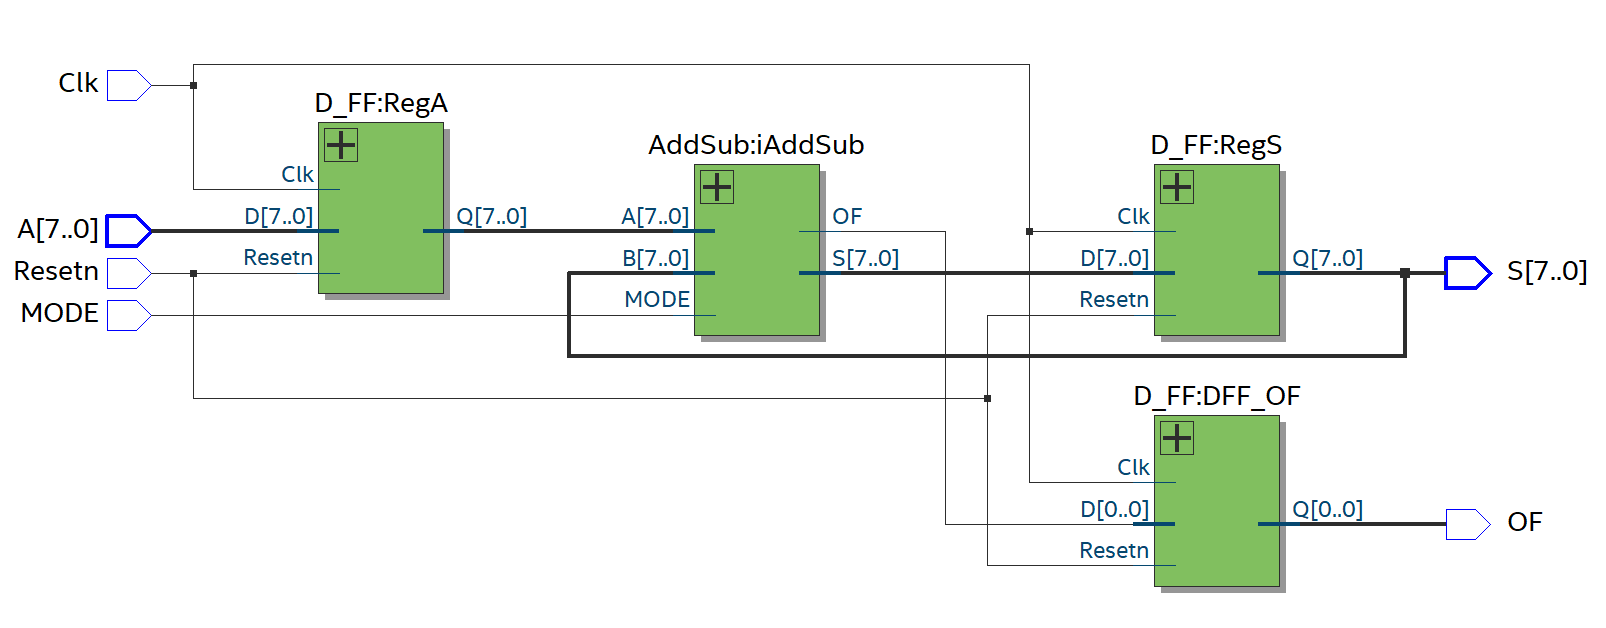
\includegraphics[width=\textwidth]{assets/ripple_addsub_rtl.png}
  \caption{RTL Viewerで表示した8ビット符号付き加減算器の回路図}
  \label{fig:ripple_addsub_rtl}
\end{figure}

次に記述したソースコードが正しく実装できているかをシミュレーションを通して確認する.
シミュレーション結果を図\ref{fig:result_adder_of0}~\ref{fig:result_sub_of1}に示す.

\begin{figure}[H]
  \centering
  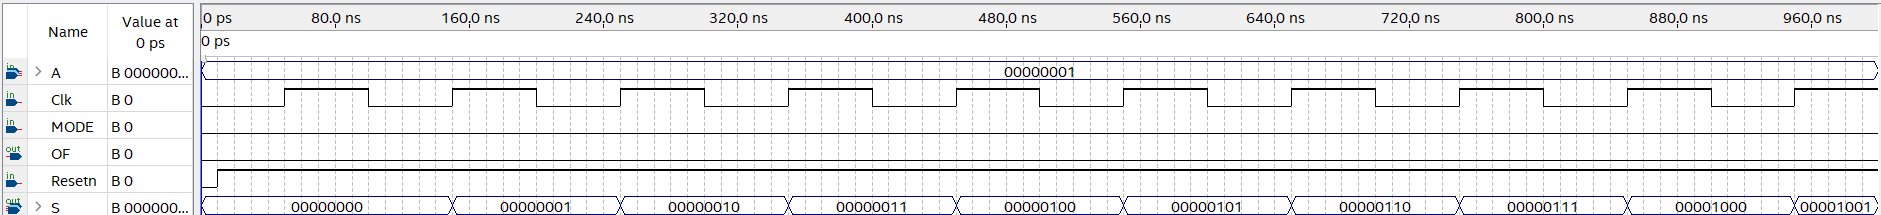
\includegraphics[width=\textwidth]{assets/add_A_1_OF_0.png}
  \caption{加算器のシミュレーション(オーバーフローなし)}
  \label{fig:result_adder_of0}
\end{figure}

\begin{figure}[H]
  \centering
  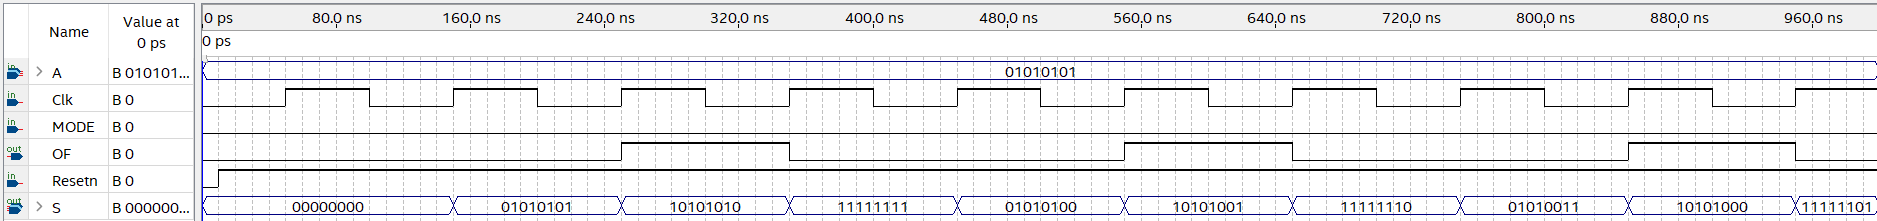
\includegraphics[width=\textwidth]{assets/add_A_01010101_OF_1.png}
  \caption{加算器のシミュレーション(オーバーフローあり)}
  \label{fig:result_adder_of1}
\end{figure}

\begin{figure}[H]
  \centering
  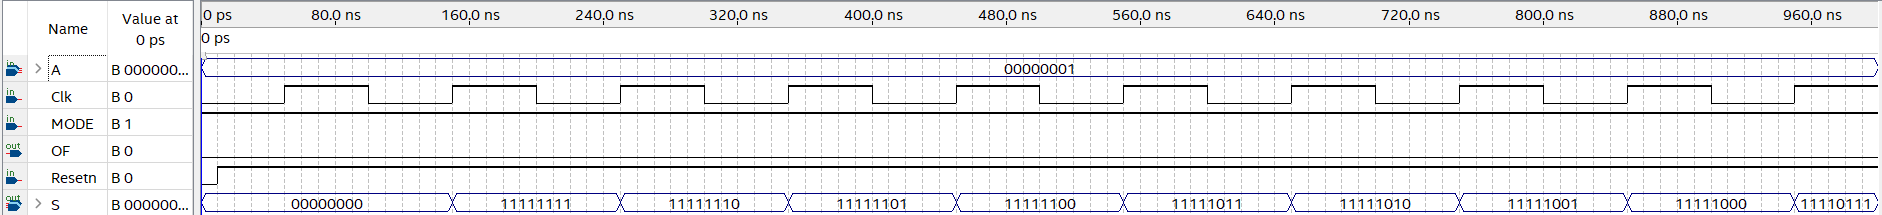
\includegraphics[width=\textwidth]{assets/sub_A_1_OF_0.png}
  \caption{減算器のシミュレーション(オーバーフローなし)}
  \label{fig:result_sub_of0}
\end{figure}

\begin{figure}[H]
  \centering
  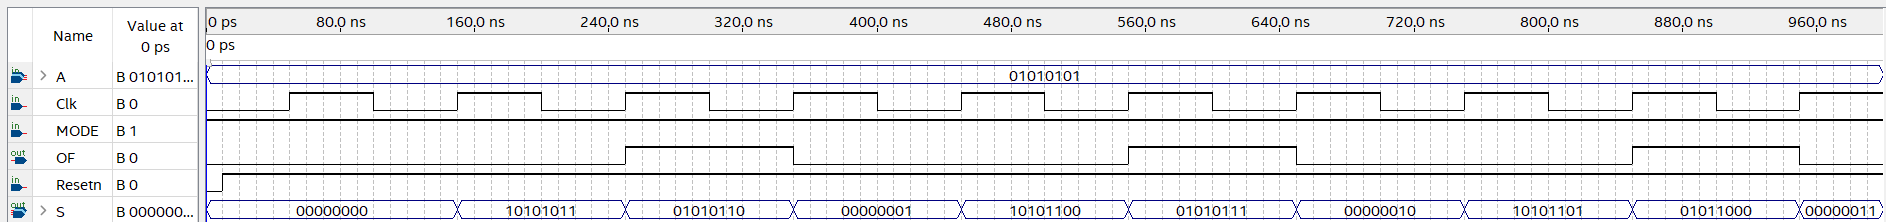
\includegraphics[width=\textwidth]{assets/sub_A_01010101_OF_1.png}
  \caption{減算器のシミュレーション(オーバーフローあり)}
  \label{fig:result_sub_of1}
\end{figure}

シミュレーション結果を順番に確認する.図\ref{fig:result_adder_of0}を見ると,
出力Sが1ずつ加算されており,オーバーフローも生じていない.また,図\ref{fig:result_adder_of1}を見ると,
2回目の加算で出力Sの符号が変わっており,OF=1となっていることから,オーバーフローが発生していることが確認できる.
したがって,加算器については実装が正しいことが確認できた.

次に減算器の確認を行う.図\ref{fig:result_sub_of0}を見ると,出力Sが1ずつ減算されており,OF=0であるためオーバーフローも生じていない.
また,図\ref{fig:result_sub_of1}を見ると,2回目の減算で出力Sの符号が反転しており,OF=1であることから
オーバーフローが発生していることが確認できる.したがって,減算器についても正しく実装が行われていることが確認できた.

\subsection{実習2}
実習1で作成した回路が動作可能な最大周波数$f_{max}$を調べた結果を図\ref{fig:fmax_ripple_addsub}に示す.
図\ref{fig:fmax_ripple_addsub}より,最大周波数$f_{max}$は$302.66[\si{\MHz}]$であることが確認できた.
\begin{figure}[H]
  \centering
  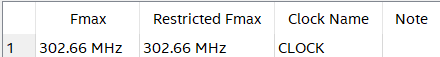
\includegraphics{assets/fmax_ripple_addsub.png}
  \caption{実習1で作成した回路が動作可能な最大周波数$f_{max}$}
  \label{fig:fmax_ripple_addsub}
\end{figure}

また,動作要求周波数($50\si{\MHz}$)におけるセットアップ時間とホールド時間が十分に確保されているかを確認した結果をそれぞれ図\ref{fig:setup_time}と図\ref{fig:hold_time}に示す.
図\ref{fig:setup_time}から,セットアップ時間に対する余裕時間は$16.696[\si{\ns}]$であることがわかる.また,図\ref{fig:hold_time}から,ホールド時間に対する余裕時間は$0.376[\si{\ns}]$であることがわかる.
\begin{figure}[H]
  \centering
  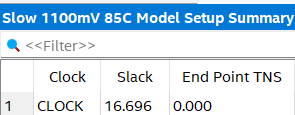
\includegraphics{assets/setup_summary.png}
  \caption{動作要求周波数($50\si{\MHz}$)におけるセットアップ時間}
  \label{fig:setup_time}
\end{figure}

\begin{figure}[H]
  \centering
  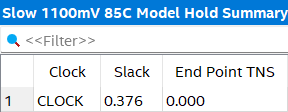
\includegraphics{assets/hold_summary.png}
  \caption{動作要求周波数($50\si{\MHz}$)におけるホールド時間}
  \label{fig:hold_time}
\end{figure}

次に,Timing Analyzerのタイミングレポートを図\ref{fig:timing_report}に,タイミングレポートから得られたクリティカルパスを図\ref{fig:critical_path}に示す.
\begin{figure}[H]
  \centering
  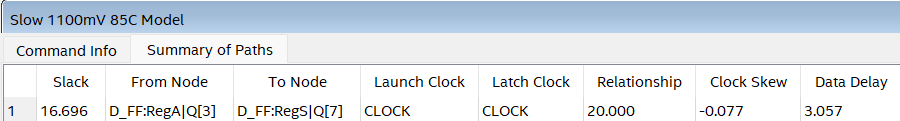
\includegraphics[width=\textwidth]{assets/critical_path_summary.png}
  \caption{Timing Analyzerのタイミングレポート}
  \label{fig:timing_report}
\end{figure}

\begin{figure}[H]
  \centering
  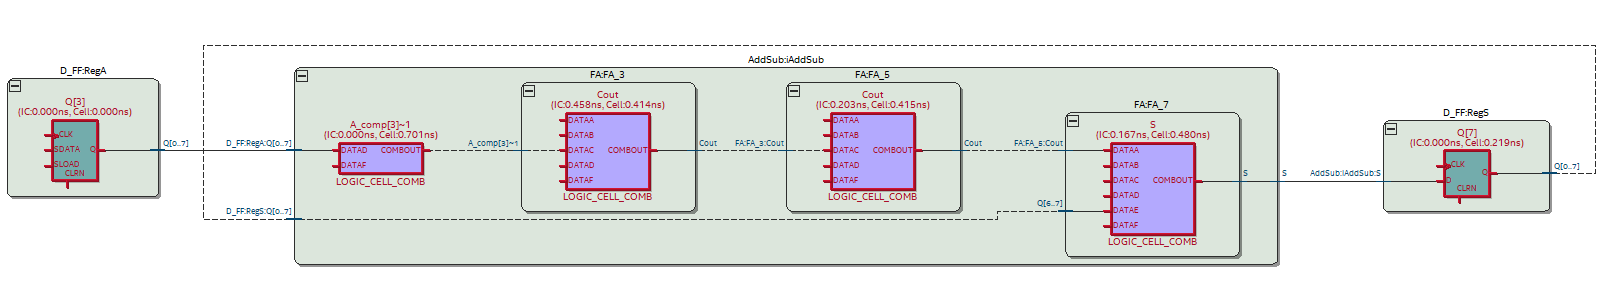
\includegraphics[width=\textwidth]{assets/timing_report_map_viewer.png}
  \caption{タイミングレポートから得られたクリティカルパス}
  \label{fig:critical_path}
\end{figure}

図\ref{fig:ripple_addsub_rtl}と図\ref{fig:critical_path}より,RegAから8ビットリプルキャリ加算減器を通って,RegSにたどり着くまでの経路がクリティカルパスであることがわかる.

\subsection{実習3}
図\ref{fig:4bit_mul_circuit}の乗算器をVerilog HDLで記述したモジュールをソースコード\ref{src:zisshu3_main}に示す.
\begin{lstlisting}[caption={乗算器のメインモジュール}, label={src:zisshu3_main}]
module multiplier(Clk, Resetn, ST, X, Y, M, x1, x2, y, m1, m2);
	input Clk, Resetn;
	input [3:0] X, Y;
	output [7:0] M;
	output [2:0] ST;
	output [6:0] x1, x2, y, m1, m2;
	wire [7:0] RegX_out, RegY_out, RegM_out, Adder_out;
	reg [7:0] RegM;
	reg [1:0] ModeX, ModeY, ModeM;
	reg [2:0] cur_st, next_st;
	
	// State
	parameter I  = 3'b000,
				 A0 = 3'b001,
				 A1 = 3'b010,
				 A2 = 3'b011,
				 A3 = 3'b100,
				 F  = 3'b101;
				 
	// Mode
	parameter LOAD    = 2'b00,
				 SHIFT_R = 2'b01,
				 SHIFT_L = 2'b10,
				 HOLD    = 2'b11;
				 
	assign ST = cur_st;
	assign M = RegM_out;
	
	always @(posedge Clk or negedge Resetn) begin
		if(!Resetn)
			cur_st <= I;
		else
			cur_st <= next_st;
		
		case(cur_st)
			I :
				begin
					ModeX   <= LOAD;
					ModeY   <= LOAD;
					ModeM   <= LOAD;
					next_st <= A0;
				end
			A0:
				begin
					ModeX   <= SHIFT_L;
					ModeY   <= SHIFT_R;
					ModeM   <= LOAD;
					next_st <= A1;
				end
			A1:
				begin
					ModeX   <= SHIFT_L;
					ModeY   <= SHIFT_R;
					ModeM   <= LOAD;
					next_st <= A2;
				end
			A2:
				begin
					ModeX   <= SHIFT_L;
					ModeY   <= SHIFT_R;
					ModeM   <= LOAD;
					next_st <= A3;
				end
			A3:
				begin
					ModeX   <= SHIFT_L;
					ModeY   <= SHIFT_R;
					ModeM   <= LOAD;
					next_st <= F;
				end
			F :
				begin
					ModeX   <= HOLD;
					ModeY   <= HOLD;
					ModeM   <= HOLD;
					next_st <= F;
				end
		endcase
	end
	
	Register RX(Clk, Resetn, X, ModeX, RegX_out);
	Register RY(Clk, Resetn, Y, ModeY, RegY_out);
	Adder ADD(RegX_out, RegM_out, RegY_out[0], Adder_out);
	Register RM(Clk, Resetn, Adder_out, ModeM, RegM_out);
	
	decoder LED_X2(RegX_out[3:0], x2);
	decoder LED_X1(RegX_out[7:4], x1);
	decoder LED_Y(RegY_out, y);
	decoder LED_M2(RegM_out[3:0], m2);
	decoder LED_M1(RegM_out[7:4], m1);
endmodule
\end{lstlisting}

また,下位モジュールについてソースコード\ref{src:register}~\ref{src:decoder}に示す.
\begin{lstlisting}[caption={モードの情報を含んだレジスタモジュール}, label={src:register}]
module Register(Clk, Resetn, D, Mode, Q);
	input Clk, Resetn;
	input [7:0] D;
	input [1:0] Mode;
	output reg [7:0] Q;
	
	// Mode
	parameter LOAD    = 2'b00,
				 SHIFT_R = 2'b01,
				 SHIFT_L = 2'b10,
				 HOLD    = 2'b11;
	
	always @(posedge Clk or negedge Resetn) begin
		if(!Resetn)
			Q <= 0;
		else
			case(Mode)
				LOAD	 : Q <= D;
				SHIFT_R: Q <= Q >> 1;
				SHIFT_L: Q <= Q << 1;
				HOLD	 : Q <= Q;
				default: Q <= 8'bxxxxxxxx;
			endcase
	end
endmodule
\end{lstlisting}

\begin{lstlisting}[caption={加算器モジュール}, label={src:adder}]
module Adder(Add, Base, Cmp, Q);
	input [7:0] Add, Base;
	input Cmp;
	output [7:0] Q;
	
	assign Q = (Cmp) ? Add + Base : Base;
endmodule
\end{lstlisting}

\begin{lstlisting}[caption={デコーダモジュール}, label={src:decoder}]
module decoder(D, Q);
	input [3:0] D;
	output [6:0] Q;
	reg [6:0] Q;
	
	always @(D) begin
		case (D)
			4'b0000: Q = 7'b1000000;
			4'b0001: Q = 7'b1111001;
			4'b0010: Q = 7'b0100100;
			4'b0011: Q = 7'b0110000;
			4'b0100: Q = 7'b0011001;
			4'b0101: Q = 7'b0010010;
			4'b0110: Q = 7'b0000010;
			4'b0111: Q = 7'b1011000;
			4'b1000: Q = 7'b0000000;
			4'b1001: Q = 7'b0010000;
			4'b1010: Q = 7'b0001000;
			4'b1011: Q = 7'b0000011;
			4'b1100: Q = 7'b1000110;
			4'b1101: Q = 7'b0100001;
			4'b1110: Q = 7'b0000110;
			4'b1111: Q = 7'b0001110;
			default: Q = 7'bxxxxxxx;
		endcase
	end
endmodule

\end{lstlisting}

RTL Viewerを用いて表示した回路図を図\ref{fig:multi_rtl}に示す.
\begin{figure}[H]
  \centering
  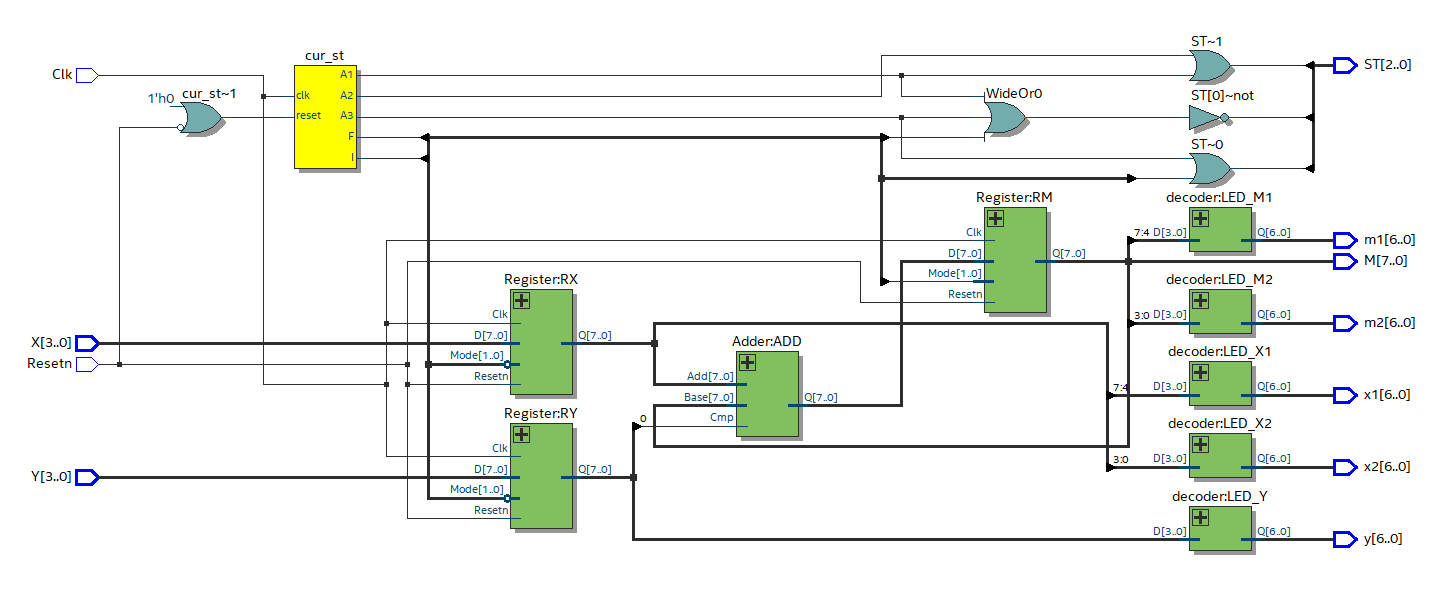
\includegraphics[width=\textwidth]{assets/multi_rtl.png}
  \caption{RTL Viewerで表示させた乗算器回路}
  \label{fig:multi_rtl}
\end{figure}

最大動作周波数を図\ref{fig:fmax_multi}に示す.
\begin{figure}[H]
  \centering
  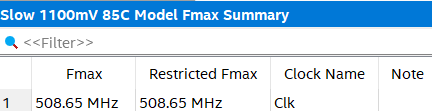
\includegraphics{assets/multi_fmax.png}
  \caption{実装した乗算器の最大動作周波数}
  \label{fig:fmax_multi}
\end{figure}


今回も時間の都合で実機実験が行えなかったため,シミュレーションで動作確認を行う.
$B \times 3$の計算シミュレーションを行った結果を図\ref{fig:result_multi_XB_Y3}に示す.なお,シミュレーションで状態の変遷が見れるように
信号STを出力している.
\begin{figure}[H]
  \centering
  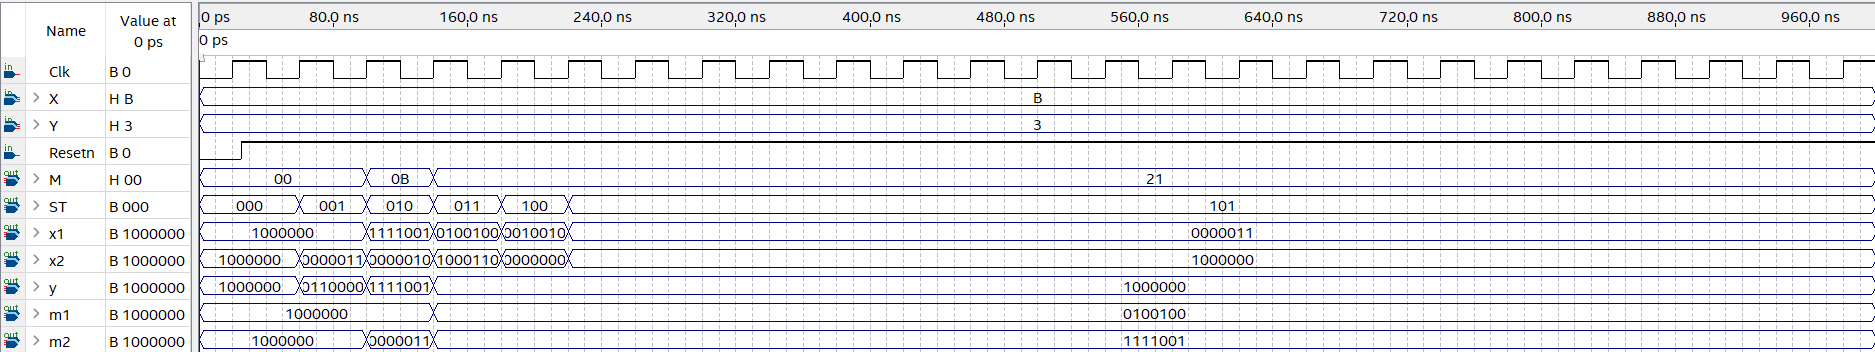
\includegraphics[width=\textwidth]{assets/multi_XB_Y3.png}
  \caption{4ビット乗算器のシミュレーション結果($B \times 3$の計算)}
  \label{fig:result_multi_XB_Y3}
\end{figure}
図\ref{fig:result_multi_XB_Y3}を見ると,最初にリセット入力で状態がIになった後,
4つの状態を辿ってから,最後の状態に移行してから定常状態となった.このとき,演算結果は$21_{(16)}$であることがわかる.
また,7セグメントディスプレイへの出力のつもりで用意しているx1,x2,y,m1,m2の値と,ソースコード\ref{src:decoder}を見比べると,
きちんと数字が反映されており,演算結果とも正しいことが分かる.したがって,実装は正しいことが確認できた.

\subsection{実習4}
被乗数$X$を負の数も使えるようにするには,先頭の4ビットに1111を付与すればいいため,ソースコード\ref{src:zisshu3_main}で``Register RX(Clk, Resetn, X, ModeX, RegX\_out);''と記述していたものを
ソースコード\ref{src:multi_ex}のように置き換えればよい.
\begin{lstlisting}[caption={被乗数Xを負の数も使えるように拡張したもの}, label={src:multi_ex}]
  Register RX_ex (Clk, Resetn, {{4{X[3]}}, X}, ModeX, RegX_out);
\end{lstlisting}
これは,MSBの符号を取り出して,先頭の4ビットに付け足している.これにより被乗数Xの拡張が行える.

このときのシミュレーション結果を図\ref{fig:multi_ex_X-7_Y6}に示す.
\begin{figure}[H]
  \centering
  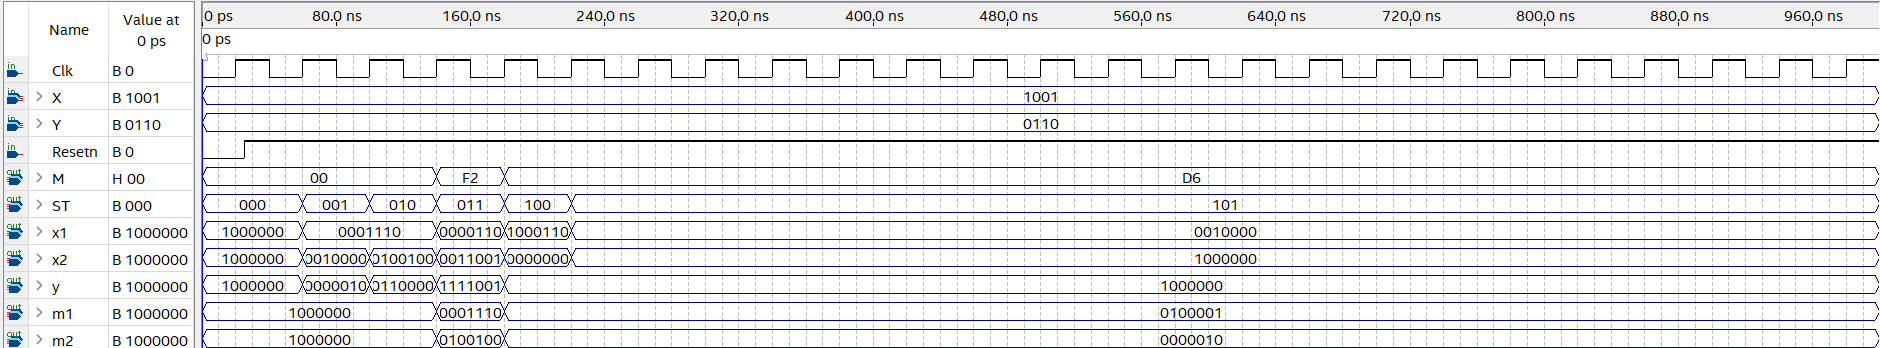
\includegraphics[width=\textwidth]{assets/multi_ex_X-7_Y6.png}
  \caption{$-7 \times 6$の演算結果}
  \label{fig:multi_ex_X-7_Y6}
\end{figure}
図\ref{fig:multi_ex_X-7_Y6}を見ると,$(1001)_2 \times (0110)_2 = (D6)_{16}$となっており,
$(1001)_2 = (-7)_{10}, (0110)_2 = (6)_{10}, (D6)_{16} = (-42)_{10}$であるため,正しい計算結果が得られていることが分かる.
したがって,拡張実装は正しく行うことが出来た.

\section{考察}
加算器と乗算器のハードウェアの設計を正しく行うことができた.
実機実験は出来なかったが,シミュレーションはどれも期待通りの結果が得られた.
回路の最大動作周波数やクリティカルパスについての知見を得ることができた.
回路の最大動作周波数を高くするためには,ゲートの段数を減らしたりすることで回路の最適化を行うのが
いいことが分かった.

\begin{thebibliography}{9}
  \bibitem{exp_text} 布目 淳.プロジェクト実習Ⅲ 論理設計 実験テキスト.京都工芸繊維大学,2024年
  \bibitem{user_manual} Terasic Technologics Inc.:  ``DE1-SoC User Manual V2.0.4'' Chapter3. Using the DE1-SoC Board, 2019
  \bibitem{logical_circuit_text} 柴山 潔.コンピュータサイエンスで学ぶ論理回路とその設計 2.3節「組み合わせ回路の最適化設計」.近代科学社,2021年
\end{thebibliography}

\end{document}